\section{Research Through Design}

\section{User-Centered Design}
\label{sec:user-centered-design}

\section{Design and Evaluation of User Interface Authoring Tools}

\textcite{Olsen:2007} argues that user interface design tools, particularly those that deal with unconventional interaction techniques (e.g. mid-air gesture sensing), do not lend themselves to conventional software evaluation methods. One reason for this is that such tools require domain-specific expertise, which --- by the nature of novel tools --- no user population possesses. Another reason is that these tools support complex tasks with high inter-user variability in terms of the users’ mental models of the tasks. “Meaningful comparisons between two tools for a realistically complex problem are confounded in so many ways as to make statistical comparisons more fantasy than fact.” \parencite{Olsen:2007} From the framework proposed by Olsen for the evaluation of user interface toolkits, I derived the following four guidelines to direct the design of my mid-air gesture authoring tool:

\begin{itemize}
\item \emph{Reduce development time.} A good authoring tool should allow for the rapid implementation of design changes. This can be encouraged by reducing the number of choices that have to be made to express a design. (Granted, there may exist a tradeoff between this concern and the expressive power of the authoring tool.)
\item \emph{Encapsulate and simplify expertise.} Considerable technical know-how is required to design and develop applications for emerging technologies. A good design tool liberates the designer from the need for prior knowledge, yet communicates the capabilities and limitations of the technology to nudge the designer towards feasible designs.
\item \emph{Lower skill barriers.} Empowering new populations of users to envision and implement designs “expands the set of people who can effectively create new applications.” \parencite{Olsen:2007}
\item \emph{Make use of a common infrastructure.} It is difficult to get users to adopt a new standard. As much as possible, authoring tools should hook up to existing and widely adopted tools and practices, and complement existing workflows; upgrading rather than negating the common denominator.
\end{itemize}

Employing a user interface paradigm for expressing design choices that reflects the problem being solved and embodies the constraints of the design space \parencite{Norman:1993} serves all four the guidelines above.

In addition, \textcite{Shoemaker:2010} propose design guidelines for body-centric interaction with large displays. From among the guidelines they propose, two generalize to influence the design of an authoring tool for mid-air gestures:

\begin{itemize}
\item Interaction using mid-air gestures at a distance should be \emph{“mediated through a representation that binds personal and extrapersonal space.”} A means for communicating the constraints and opportunities of the interaction space to the user is recommended for mid-air gestural interfaces. This holds for design tools that target these interactions.
\item It is recommended that \emph{users’ sense of proprioception be leveraged} by allowing some operations to be performed in the user’s personal space, without requiring visual feedback. In terms of authoring interactions, this guideline calls for encouraging gesture designs that capitalize on proprioception through the nature of the authoring paradigm.
\end{itemize}

In sum, six guidelines derived from previous work form the basis of my design rationale for the gesture authoring interface (Figure~\ref{fig:design-guidelines}). The first four, derived from \posscite{Olsen:2007} work, identify and address concerns that pertain to user interface design tools. The last two, derived from the work of \textcite{Shoemaker:2010}, attend to concerns related to perceptual interactions in general. Whether or not the final design for the authoring tool conforms to these guidelines is evaluated through user studies.

\begin{SCfigure}[\sidecaptionrelwidth][ht]
\centering
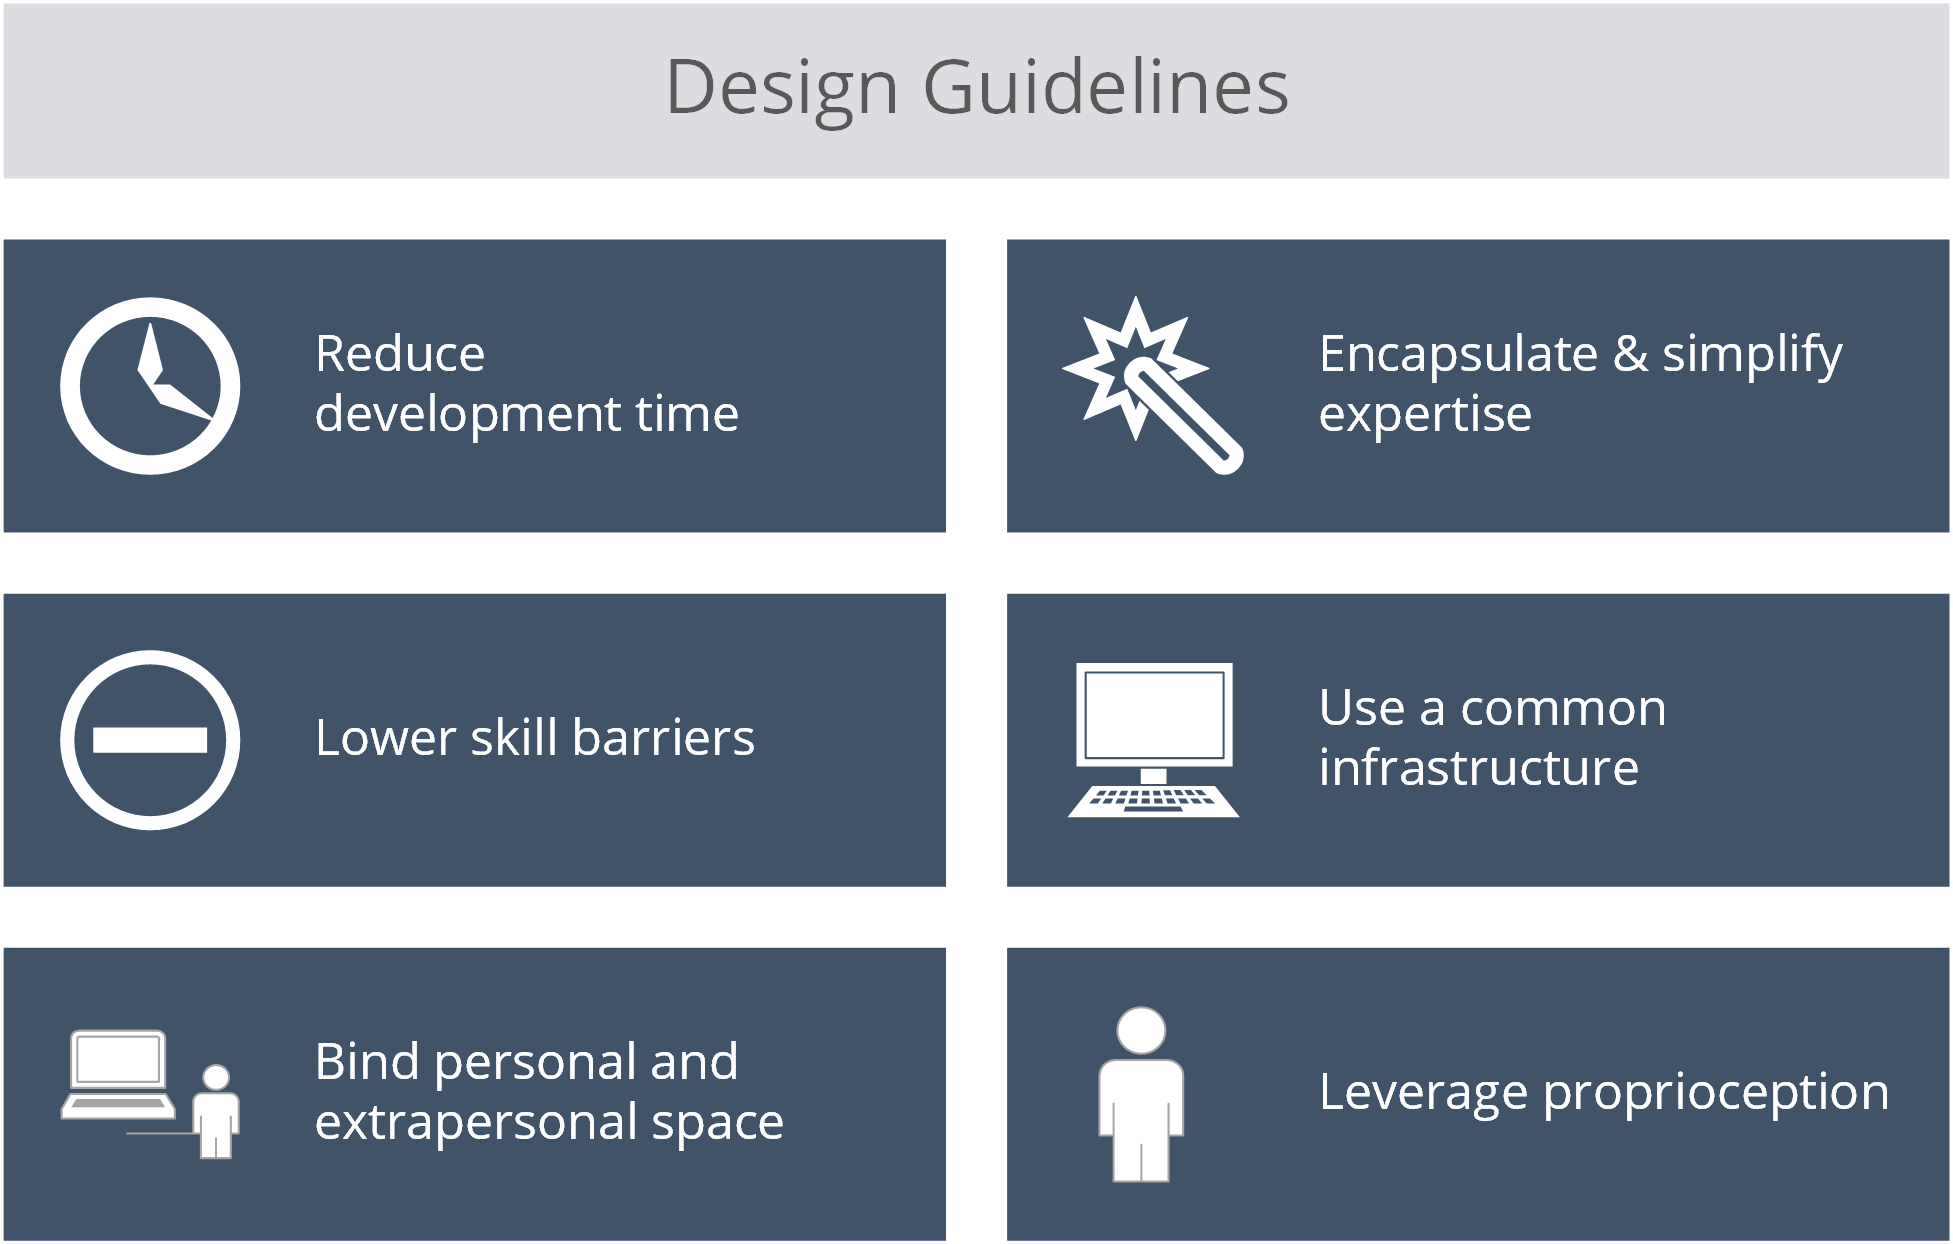
\includegraphics[width=0.7\textwidth]{design-guidelines}
\caption{Guidelines derived from the literature formed the basis of the design rationale for a gesture authoring tool.}
\label{fig:design-guidelines}
\end{SCfigure}

Additionally, from a programming perspective (see Section~\ref{sec:end-user-programming}); \textcite{Myers:2000} identify five themes that influence the success of user interface tools:

\begin{itemize}
\item User interface tools should strive to achieve a low \emph{threshold} --- i.e. be easy to learn --- and a high \emph{ceiling} --- i.e. significant expressive power.
\item Successful tools lead users to making the right choices and avoiding wrong designs by offering a well-designed \emph{path of least resistance}
\item A tool should embody \emph{predictability} and avoid unpredictable automatic operations.
\item Developers of user interface tools should stay on top of developments, since user interface technologies are \emph{moving targets} that can change significantly or become obsolete at a rapid pace.
\item A tool should only \emph{address the parts of the user interface that are needed}.
\end{itemize}

The first of these themes is specifically captured in part by Olsen's recommendations that a tool should lower skill barriers and empower new users. A high level of expressive power is desirable, but the weight of this concern will be governed by user needs (see Section~\ref{sec:user-centered-design}). The encapsulation and simplification of expertise, along with the use of user-centered design tools and methods, integrate all of these themes.
